\documentclass[12pt]{article}
\newif\ifanswer%\answertrue% comment out \answertrue to show/hide answers
\usepackage{../../preamble3}% preamble always after \newif\ifanswer
%\pagenumbering{gobble}
\title{MathCounts State Competition, March 25, 2021 \\ Sprint Round}
\author{Patrick \& James Toche}
\date{Revised:~\today}

\begin{document}
\maketitle
\begin{minipage}{\textwidth}
\begin{abstract}\setlength{\parindent}{0pt}%
Notes on the State Competition, March 25, 2021. 
Questions are from MathCounts Foundation (\url{https://www.mathcounts.org/}). Copyright restrictions may apply. Written for personal use. 
Please report typos and errors over at \url{https://github.com/ptoche/Math/tree/master/mathcounts}. 
\end{abstract}
\end{minipage}

\thispagestyle{empty}
\clearpage

\section*{Sprint Round}

%%%%%%%%%%%%%%%%%%%%%%%%%%%%%%%%%%%%%%%%%%%%%%%%%%%%%%%%%%%%%%%%%%%%%%%%
\subsection*{1.}

\nopagebreak

Holly is selling candy bars to raise money for her softball team. She starts with $80$ candy bars and sells $32$ to her neighbors and $15$ to her grandparents. How many candy bars does Holly have left to sell? 

\fbox{\phantom{ANSWER}}~candy bars

\begin{answer}
\begin{align*}
80 - 32 - 15  = 33
\end{align*}
\begin{empheq}[box={\mathbox[colback=white]}]{equation*}
    33 ~\text{candy bars}
\end{empheq} 
\end{answer}
%%%%%%%%%%%%%%%%%%%%%%%%%%%%%%%%%%%%%%%%%%%%%%%%%%%%%%%%%%%%%%%%%%%%%%%%

\iftoggle{showAnswers}{\newpage}

%%%%%%%%%%%%%%%%%%%%%%%%%%%%%%%%%%%%%%%%%%%%%%%%%%%%%%%%%%%%%%%%%%%%%%%%
\subsection*{2.}

\nopagebreak

A recipe for chocolate chip cookies calls for $2\sfrac{1}{4}$ cups of chocolate chips. Jaime only has $\sfrac{1}{4}$ cup measuring cup. To measure the exact amount of chocolate chips needed for the recipe, how many times does Jaime need to fill up the measuring cup? 

\fbox{\phantom{ANSWER}}~times

\begin{answer}
\begin{align*}
2 \sfrac{1}{4} 
  = 2 + \frac{1}{4}
  = \frac{9}{4} 
  = 9 \times \frac{1}{4}
\end{align*}
\begin{empheq}[box={\mathbox[colback=white]}]{equation*}
    9 ~\text{times}
\end{empheq} 
\end{answer}
%%%%%%%%%%%%%%%%%%%%%%%%%%%%%%%%%%%%%%%%%%%%%%%%%%%%%%%%%%%%%%%%%%%%%%%%

\iftoggle{showAnswers}{\newpage}

%%%%%%%%%%%%%%%%%%%%%%%%%%%%%%%%%%%%%%%%%%%%%%%%%%%%%%%%%%%%%%%%%%%%%%%%
\subsection*{3.}

\nopagebreak

If $0.0036$ divided by $n$ is equal to $0.000012$, what is the value of $n$?

\fbox{\phantom{ANSWER}}

\begin{answer}
\begin{align*}
\frac{0.0036}{n} 
  & = 0.000012 \\[2ex]
\Rightarrow \quad
 n & = 
\frac{0.0036}{0.000012 } 
  = \frac{3600}{12}
  = 300
\end{align*}
\begin{empheq}[box={\mathbox[colback=white]}]{equation*}
    300
\end{empheq} 
\end{answer}
%%%%%%%%%%%%%%%%%%%%%%%%%%%%%%%%%%%%%%%%%%%%%%%%%%%%%%%%%%%%%%%%%%%%%%%%

\iftoggle{showAnswers}{\newpage}

%%%%%%%%%%%%%%%%%%%%%%%%%%%%%%%%%%%%%%%%%%%%%%%%%%%%%%%%%%%%%%%%%%%%%%%%
\subsection*{4.}

\nopagebreak
Alonzo draws a diagonal of a convex polygon with $8$ sides. The diagonal divides the polygon into two smaller polygons, one with $6$ sides and one with $n$ sides. What is the value of $n$?

\fbox{\phantom{ANSWER}}

\begin{answer}
As you connect two diagonals of a polygon, you get two extra sides. 
\begin{center}
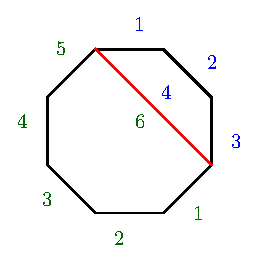
\includegraphics[height=7cm,page=1]{sprint-03-figure}
\end{center}
\begin{align*}
\text{sum of \# sides} = 8 + 2 & = 10 \\
\text{sum of \# sides} = 6 + n & = 10 \\
\Rightarrow 
n & = 4
\end{align*}
\begin{empheq}[box={\mathbox[colback=white]}]{equation*}
    4
\end{empheq} 
\end{answer}
%%%%%%%%%%%%%%%%%%%%%%%%%%%%%%%%%%%%%%%%%%%%%%%%%%%%%%%%%%%%%%%%%%%%%%%%

\iftoggle{showAnswers}{\newpage}

%%%%%%%%%%%%%%%%%%%%%%%%%%%%%%%%%%%%%%%%%%%%%%%%%%%%%%%%%%%%%%%%%%%%%%%%
\subsection*{5.}

\nopagebreak

When $x=3$, what is the value of the expression $4^{\displaystyle x-5}$~? Express your answer as a common fraction.

\begin{minipage}[b]{\linewidth}
\fbox{\phantom{ANSWER}}\\
\mbox{---------------}\\
\fbox{\phantom{ANSWER}}
\end{minipage}

\begin{answer}
Substitute $x$ with $3$:
\begin{align*}
4^{3-5} = 4^{-2} = \frac{1}{4^2} = \frac{1}{16}
\end{align*}
\begin{empheq}[box={\mathbox[colback=white]}]{equation*}
    \frac{1}{16}
\end{empheq} 
\end{answer}
%%%%%%%%%%%%%%%%%%%%%%%%%%%%%%%%%%%%%%%%%%%%%%%%%%%%%%%%%%%%%%%%%%%%%%%%


\iftoggle{showAnswers}{\newpage}

%%%%%%%%%%%%%%%%%%%%%%%%%%%%%%%%%%%%%%%%%%%%%%%%%%%%%%%%%%%%%%%%%%%%%%%%
\subsection*{6.}

\nopagebreak

Sylvia the snail crawls $23$ inches in the first hour, then $59$ inches in the second hour, then $49$ inches in the third hour. How many feet does Sylvia crawl in these three hours? Express your answer to the nearest whole number

\fbox{\phantom{ANSWER}}~ft

\begin{answer}
We could add it all up and then convert to feet
\begin{align*}
23 + 59 + 49 = 131
\end{align*}
but that involves dividing $131$ by $12$: $131=10\times12+11$. To avoid this large division, we can instead convert the smaller numbers first and add at the last step:
\begin{align*}
& \hspace{38pt} 23~\text{in} 
  \longrightarrow 2~\text{ft} - 1~\text{in}\\
& +\qquad 59~\text{in} 
  \longrightarrow 5~\text{ft} - 1~\text{in}\\
& +\qquad 49~\text{in} 
  \longrightarrow 4~\text{ft} + 1~\text{in}\\
\cline{1-2}
& =~\quad 131~\text{in} 
  \longrightarrow 11~\text{ft} - 1~\text{in} 
\end{align*}
\begin{empheq}[box={\mathbox[colback=white]}]{equation*}
    11 ~\text{ft}
\end{empheq} 
\end{answer}
%%%%%%%%%%%%%%%%%%%%%%%%%%%%%%%%%%%%%%%%%%%%%%%%%%%%%%%%%%%%%%%%%%%%%%%%


\iftoggle{showAnswers}{\newpage}

%%%%%%%%%%%%%%%%%%%%%%%%%%%%%%%%%%%%%%%%%%%%%%%%%%%%%%%%%%%%%%%%%%%%%%%%
\subsection*{7.}

\nopagebreak

Ben, Rachel and Teri collected seashells on a beach. Ben collected five more than twice as many seashells as Teri collected. Rachel collected seven less than four times as many seashells as Teri collected. If Ben and Rachel collected the same number of seashells, how many seashells did Teri collect?

\fbox{\phantom{ANSWER}}

\begin{answer}
Let $B$ denote seashells collected by Ben, $T$ seashells collected by Teri, and $R$ seashells collected by Rachel. The question can be translated as the following system:
\begin{align*}
B & = 5 + 2T\\
R & = 4T - 7\\
B & = R
\end{align*}
Substituting $R$ out, we can solve for $T$:
\begin{align*}
5 + 2T & = 4T - 7 \\
     T & = \frac{12}{2} = 6
\end{align*}
\begin{empheq}[box={\mathbox[colback=white]}]{equation*}
    6
\end{empheq} 
\end{answer}
%%%%%%%%%%%%%%%%%%%%%%%%%%%%%%%%%%%%%%%%%%%%%%%%%%%%%%%%%%%%%%%%%%%%%%%%

\iftoggle{showAnswers}{\newpage}

%%%%%%%%%%%%%%%%%%%%%%%%%%%%%%%%%%%%%%%%%%%%%%%%%%%%%%%%%%%%%%%%%%%%%%%%
\subsection*{8.}

\nopagebreak

At Kickin' Chicken, a chicken sandwich costs $\$4$, plus $7\%$ sales tax. If Quincy orders a chicken sandwich and pays with a $\$20$ bill, how much change will he receive?

\$~\fbox{\phantom{ANSWER}}

\begin{answer}
The total amount paid, including tax, is
\begin{align*}
4 \times 1.07 = 4.28
\end{align*}
and thus the amount of change:
\begin{align*}
20 - 4.28 = 15.72
\end{align*}
\begin{empheq}[box={\mathbox[colback=white]}]{equation*}
    \$ 15.72
\end{empheq} 
\end{answer}
%%%%%%%%%%%%%%%%%%%%%%%%%%%%%%%%%%%%%%%%%%%%%%%%%%%%%%%%%%%%%%%%%%%%%%%%

\iftoggle{showAnswers}{\newpage}

%%%%%%%%%%%%%%%%%%%%%%%%%%%%%%%%%%%%%%%%%%%%%%%%%%%%%%%%%%%%%%%%%%%%%%%%
\subsection*{9.}

\nopagebreak

In right triangle ABC, point D is on side BC, as shown. If $\text{BC}=5\times BD$ and the area of $\Delta ABD$ is $8$~in$^2$, what is the area of $\Delta ABC$? 

\begin{center}
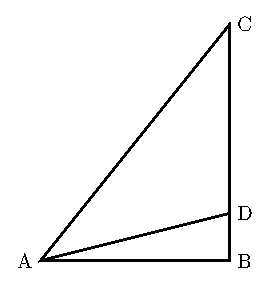
\includegraphics[height=5cm,page=1]{sprint-09-figure}
\end{center}

\fbox{\phantom{ANSWER}}~in$^2$

\begin{answer}
The areas of triangles ABC and ABD are:
\begin{align*}
\Delta \text{ABC} = \frac{1}{2} \times \text{AB} \times \text{BC} \\
\Delta \text{ABD} = \frac{1}{2} \times \text{AB} \times \text{BD} 
\end{align*}
There's an obvious common factor, which means the ratios will be simpler. Let's divide these:
\begin{align*}
\frac{\Delta \text{ABC}}{\Delta \text{ABD}} 
  = \frac{\text{BC}}{\text{BD}} 
& = 5 \\[2ex]
\Rightarrow \quad
\Delta \text{ABC}
& = 5 \times 8 
  = 40
\end{align*}
\begin{empheq}[box={\mathbox[colback=white]}]{equation*}
    40 ~\text{in}^2
\end{empheq} 
\end{answer}
%%%%%%%%%%%%%%%%%%%%%%%%%%%%%%%%%%%%%%%%%%%%%%%%%%%%%%%%%%%%%%%%%%%%%%%%

\iftoggle{showAnswers}{\newpage}

%%%%%%%%%%%%%%%%%%%%%%%%%%%%%%%%%%%%%%%%%%%%%%%%%%%%%%%%%%%%%%%%%%%%%%%%
\subsection*{10.}

\nopagebreak

By selling handmade dolls, Hannah hopes to earn at least $\$1500$ to donate to the local hospital. If she makes between $\$40$ and $\$90$ for each doll she sells, what is the absolute difference between the minimum and maximum number of dolls she must sell to meet her minimum fundraising goal?

\fbox{\phantom{ANSWER}}~dolls

\begin{answer}
Minimum:
\begin{align*}
\frac{1500}{90} = 17
\end{align*}
Maximum:
\begin{align*}
\frac{1500}{40} = 38
\end{align*}
Difference: 
\begin{align*}
38 - 17 = 21
\end{align*}
\begin{empheq}[box={\mathbox[colback=white]}]{equation*}
    21~\text{dolls}
\end{empheq} 
\end{answer}
%%%%%%%%%%%%%%%%%%%%%%%%%%%%%%%%%%%%%%%%%%%%%%%%%%%%%%%%%%%%%%%%%%%%%%%%

\iftoggle{showAnswers}{\newpage}

%%%%%%%%%%%%%%%%%%%%%%%%%%%%%%%%%%%%%%%%%%%%%%%%%%%%%%%%%%%%%%%%%%%%%%%%
\subsection*{11.}

\nopagebreak

A fence is to be placed along the perimeter of a rectangular field with area $400\text{ft}^2$ and minimum possible perimeter. If one foot of fencing costs $\$2.50$, what is the total cost of the fencing needed to completely enclose the field? 

\fbox{\phantom{ANSWER}}

\begin{answer}
The ``efficient'' perimeter is the square: A square with area $400$ has side length $20$ and perimeter $80$. At a cost of $\$2.50$ per foot, the total cost is therefore:
\begin{align*}
80 \times \$2.50 = \$ 200
\end{align*}

Let's show that the rectangle with minimum perimeter, for a given area, is the square.

Let $a$ and $b$ denote the side lengths of the rectangle. Its area is $ab$ and perimeter $a+b$. Now minimize the perimeter subject to the constraint that the area is some number $A$. In mathematical notation:
\begin{align*}
\min (a+b) ~\text{such that}~ ab = A
\end{align*}
By substituting $b$ out, the problem may be simplified:
\begin{align*}
\min \left(a+\frac{A}{a}\right)
\end{align*}
where $A$ is a given constant (the area) and $a$ the unknown of the reduced problem (one of the sides of the rectangle, the other being $b=A/a$). What is the value of $a$ that minimizes this quantity? 

There is a tradeoff: The first part of the sum, $a$, is increasing in $a$ linearly. The second part of the sum, $A/a$, is decreasing in $a$ at a non-linear rate. The minimum is achieved where changes in $a$ have canceling effects on the first part and second part (think about why that is true). Let a small increase in $a$ be denoted $da$. With an increase of $da$, the first part increases by exactly $da$, while the second part decreases by
\begin{align*}
\frac{A}{a} - \frac{A}{a+da}
 = A\left(\frac{1}{a}-\frac{1}{a+da}\right)
 = A\left(\frac{a+da-a}{a(a+da)}\right) 
 = \frac{Ada}{a(a+da)}
\end{align*}
We want the two effects to cancel each other out:
\begin{align*}
da  = \frac{Ada}{a(a+da)}
\end{align*}
Solve for $a$ in terms of $da$ and let $da\rightarrow 0$:
\begin{align*}
a(a+da) & = A \\
a^2 & = A \qquad \text{as}~ da \rightarrow 0
\end{align*}
which is of course the formula for the area of a square with side length $a$, implying $a=b$.

What we did above in letting $da\rightarrow0$ is calculus without the shortcut of differentiation.

In the special case $A=400$, $a=\sqrt{400}=20$, as we stated earlier. 

\begin{empheq}[box={\mathbox[colback=white]}]{equation*}
    \$200
\end{empheq} 
\end{answer}
%%%%%%%%%%%%%%%%%%%%%%%%%%%%%%%%%%%%%%%%%%%%%%%%%%%%%%%%%%%%%%%%%%%%%%%%

\iftoggle{showAnswers}{\newpage}

%%%%%%%%%%%%%%%%%%%%%%%%%%%%%%%%%%%%%%%%%%%%%%%%%%%%%%%%%%%%%%%%%%%%%%%%
\subsection*{12.}

\nopagebreak

If each side of a square is decreased in length by $2$cm, its area is decreased by $160$cm$^2$. What is the original side length of the square?

\fbox{\phantom{ANSWER}}

\begin{answer}
Consider the figure below and the unknown $x$.
\begin{center}
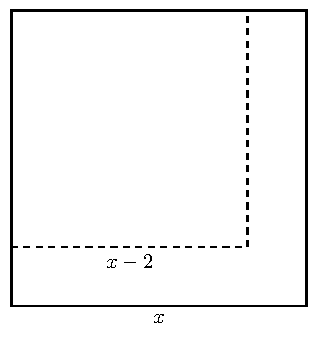
\includegraphics[height=5cm,page=1]{sprint-12-figure}
\end{center}
The area of the original square is $x^2$. The area of the smaller square is $(x-2)^2$. And the difference is
\begin{align*}
x^2 - (x-2)^2 & = 160 \\
\left(x - (x-2)\right) \times \left(x+(x-2)\right) & = 160 \\
2 \left(2x-2)\right) & = 160 \\
4(x -1) & = 160 \\
x -1 & = 40 \\
   x & = 41 
\end{align*}
Quick check:
\begin{align*}
41^2 - 39^2
  & = 41^2 - 40^2 + 40^2 - 39^2 \\
  & = (41 + 40) + (40 + 39) \\
  & = 4 \times 40 = 160 \qquad\qquad\checkmark
\end{align*}
\begin{empheq}[box={\mathbox[colback=white]}]{equation*}
    41
\end{empheq} 
\end{answer}
%%%%%%%%%%%%%%%%%%%%%%%%%%%%%%%%%%%%%%%%%%%%%%%%%%%%%%%%%%%%%%%%%%%%%%%%

\iftoggle{showAnswers}{\newpage}

%%%%%%%%%%%%%%%%%%%%%%%%%%%%%%%%%%%%%%%%%%%%%%%%%%%%%%%%%%%%%%%%%%%%%%%%
\subsection*{13.$^{\textbf{*}}$}

\nopagebreak

In Mr. Patterson's class, the average score among students who studied for an exam was $78$. The average among students who did not study was $54$. The overall class average was $70$. What portion of the class did not study? Express your answer as a common fraction. 

\begin{minipage}[b]{\linewidth}
\fbox{\phantom{ANSWER}}\\
\mbox{---------------}\\
\fbox{\phantom{ANSWER}}
\end{minipage}

\begin{answer}
Let $n$ denote the total number of students. 
Let $x_i$ denote the grade of student $i$. Let students $i=1,2,\ldots,k$ be the students who studied. And let students $i=k+1,k+2,\ldots,n$ be the students who did not study. The information we have can be stated as:
\begin{align*}
\frac{x_1 + x_2 + \ldots x_k}{k} & = 78 \\ 
\frac{x_{k+1} + x_{k+2} + \ldots x_n}{n-k} & = 54 \\ 
\frac{x_1 + x_2 + \ldots x_n}{n} & = 70 
\end{align*}
The key insight from writing the relations explicitly is that the left-hand side of the third equality can be obtained from the first two. Multiply through by the denominator:
\begin{align*}
x_1 + x_2 + \ldots x_k & = 78 k\\ 
x_{k+1} + x_{k+2} + \ldots x_n & = 54 (n-k) \\ 
x_1 + x_2 + \ldots x_n & = 70 n 
\end{align*}
Add the first two equations:
\begin{align*}
x_1 + x_2 + \ldots x_n = 78 k + 54 (n-k)
\end{align*}
Equate with the third:
\begin{align*}
78 k + 54 (n-k) = 70 n
\end{align*}
This is one linear equation in two unknowns $k$ and $n$. But recall that we are solving for the ratio of non-studying students to the total number of students, that is our unknown is 
\begin{align*}
\frac{n-k}{n}
\end{align*}
Dividing our equation by $n$ makes this unknown appear:
\begin{align*}
78 \left(\frac{k}{n}\right) + 54 \left(\frac{n-k}{n}\right) = 70
\end{align*}
At first sight this looks like a linear equation in two unknowns $\dfrac{k}{n}$ and $\dfrac{n-k}{n}$, but there is another simplification since
\begin{align*}
\frac{n-k}{n} = 1 - \frac{k}{n}
\end{align*}
We could substitute this relation back in and solve for $\dfrac{k}{n}$ or quicker still solve directly for $\dfrac{k-n}{n}$:
\begin{align*}
78 \left(1-\frac{n-k}{n}\right) + 54 \left(\frac{n-k}{n}\right) 
  & = 70\\
(78-54)\left(\frac{n-k}{n}\right) 
  & = 8\\
\left(\frac{n-k}{n}\right)  
 & = \frac{24}{8} = \frac{1}{3}
\end{align*}

Prof. Po-Shen Loh shows a quicker, more intuitive way, recommended for a competition. Think of the average of the two groups of students as weights on a scale, where the students who study are positioned on the right-hand side and the others on the left-hand side. The overall average, $70$, gives the position of where the scales are balanced (equivalently, the ``center of gravity'' or more appropriately in this case, the ``barycenter''). Relative to $70$, the weight on the left-hand side is short by $16$, while the weight on the right-hand side is in excess by $8$ units.
\begin{center}
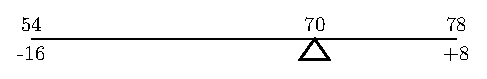
\includegraphics[width=0.7\linewidth,page=1]{sprint-13-figure}
\end{center}
This representation makes it clear that the ratio of weights on the left and right are $2{:}1$ (since $16=2\times8$), implying a fraction of:
\begin{empheq}[box={\mathbox[colback=white]}]{equation*}
    \frac{1}{3}
\end{empheq} 
\end{answer}
%%%%%%%%%%%%%%%%%%%%%%%%%%%%%%%%%%%%%%%%%%%%%%%%%%%%%%%%%%%%%%%%%%%%%%%%

\iftoggle{showAnswers}{\newpage}

%%%%%%%%%%%%%%%%%%%%%%%%%%%%%%%%%%%%%%%%%%%%%%%%%%%%%%%%%%%%%%%%%%%%%%%%
\subsection*{14.}

\nopagebreak

Forty balls, numbered $1$ to $40$, are placed in a bag. What is the probability that the number on a randomly drawn ball is a multiple of $4$ or $5$? Express your answer as a common fraction. 

\begin{minipage}[b]{\linewidth}
\fbox{\phantom{ANSWER}}\\
\mbox{---------------}\\
\fbox{\phantom{ANSWER}}
\end{minipage}

\begin{answer}
The numbers $4$ and $5$ are relatively prime, so that the probability of being a multiple of $4$ and being a multiple of $5$ are independent, and therefore their marginal probabilities may be multiplied together. Every $4$th number is a multiple of $4$, so a fraction $3/4$ are not. Likewise, every $5$th number is a multiple of $5$, so a fraction $4/5$ are not. 
The total probability is then
\begin{align*}
\frac{3}{4} \times \frac{4}{5} = \frac{3}{5}
\end{align*}
Why are the probabilities independent? Prof. Po-Shen Loh explains it thus. Consider the numbers from $0$ to $19$. Highlight the multiples of $4$ in red and the multiples of $5$ in blue. In this range, there is one common multiple. Among all numbers in this range, the multiples of $4$ account for a fraction of $1/4$ ($5$ multiples of $4$ out of a total of $20$ integers). Among the multiples of $5$, the multiples of $4$ also account for a fraction $1/4$ ($1$ multiple of $4$ out of a total of $5$ multiples of $5$). And among the non-multiples of $5$, again a fraction $1/4$ ($4$ multiples of $4$ out of a total of $16$ non-multiples of $5$). The same reasoning would hold for multiples of $5$: they account for a fraction of $1/5$ among all numbers, among all multiples of $4$, and among all non-multiples of $4$. In other words, ``multiple of $4$'' and ``multiple of $5$'' are independent events. 
\begin{center}
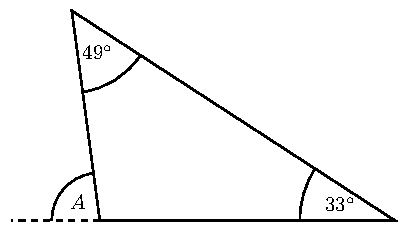
\includegraphics[height=6cm,page=1]{sprint-14-figure}
\end{center}

If you are unconvinced about the treatment of $0$ in the grid above, consider the integers from $20$ to $39$ instead. The same pattern holds:
\begin{center}
\includegraphics[height=6cm,page=2]{sprint-14-figure}
\end{center}
\begin{empheq}[box={\mathbox[colback=white]}]{equation*}
    \frac{3}{5}
\end{empheq} 
\end{answer}
%%%%%%%%%%%%%%%%%%%%%%%%%%%%%%%%%%%%%%%%%%%%%%%%%%%%%%%%%%%%%%%%%%%%%%%%

\iftoggle{showAnswers}{\newpage}

%%%%%%%%%%%%%%%%%%%%%%%%%%%%%%%%%%%%%%%%%%%%%%%%%%%%%%%%%%%%%%%%%%%%%%%%
\subsection*{15.}

\nopagebreak

\fbox{\phantom{ANSWER}}

If $3^{\displaystyle 3^{\displaystyle n}} = 27^{\displaystyle 27^{\displaystyle 27}}$, what is the value of $n$?

\begin{answer}
The key here is to rewrite $27$ as a power of $3$:
\begin{align*}
3^{\textstyle3^{\textstyle n}} 
 & = 27^{\textstyle27^{\textstyle27}} \\
 & = \left(3^3\right)^{\textstyle27^{\textstyle27}} \\
 & = 3^{\textstyle 3 \times 27^{\textstyle27}} 
\end{align*}
We can now equate the powers of $3$:
\begin{align*}
3^{n} 
  & = 3 \times 27^{\textstyle27} \\
  & = 3 \times \left(3^3\right)^{\textstyle27} \\
  & = 3^{\textstyle 1 + 3 \times 27} \\
\Rightarrow 
n & = 1 + 3 \times 27 = 81
\end{align*}
\begin{empheq}[box={\mathbox[colback=white]}]{equation*}
    81
\end{empheq} 
\end{answer}
%%%%%%%%%%%%%%%%%%%%%%%%%%%%%%%%%%%%%%%%%%%%%%%%%%%%%%%%%%%%%%%%%%%%%%%%

\iftoggle{showAnswers}{\newpage}

%%%%%%%%%%%%%%%%%%%%%%%%%%%%%%%%%%%%%%%%%%%%%%%%%%%%%%%%%%%%%%%%%%%%%%%%
\subsection*{16.}

\nopagebreak

Paloma has a bag containing red, blue, and white marbles. The ratio of red to blue marbles is $4{:}3$ and the ratio of blue to white marbles is $7{:}2$. What is the probability of Paloma randomly drawing a blue marble from this bag? Express your answer as a common fraction. 

\begin{minipage}[b]{\linewidth}
\fbox{\phantom{ANSWER}}\\
\mbox{---------------}\\
\fbox{\phantom{ANSWER}}
\end{minipage}

\begin{answer}
Let $r$ stand for red, $b$ for blue, and $w$ for white. The ratios are:
\begin{center}
\renewcommand{\arraystretch}{1.5}
\begin{tabular}{@{}C{20pt}C{10pt}C{20pt}C{10pt}C{20pt}@{}} 
\toprule
 r & : &  b & : & w \\
 4 & : &  3 &   &   \\
   &   &  7 & : & 2 \\
28 & : & 21 & : & 6 \\
\bottomrule
\end{tabular}
\end{center}
The ratio $28{:}21{:}6$ is the smallest whole-integer combination of balls that give the exact ratios given in the question. The total number of balls is (a multiple of):
\begin{align*}
28 + 21 + 6 = 55
\end{align*}
and therefore the ratio of blue marbles is $\dfrac{21}{55}$.
\begin{empheq}[box={\mathbox[colback=white]}]{equation*}
    \frac{21}{55}
\end{empheq} 
\end{answer}
%%%%%%%%%%%%%%%%%%%%%%%%%%%%%%%%%%%%%%%%%%%%%%%%%%%%%%%%%%%%%%%%%%%%%%%%

\iftoggle{showAnswers}{\newpage}

%%%%%%%%%%%%%%%%%%%%%%%%%%%%%%%%%%%%%%%%%%%%%%%%%%%%%%%%%%%%%%%%%%%%%%%%
\subsection*{17.}

\nopagebreak

Riley's entire extended family goes out to eat. Each person orders either a salad for $\$6.50$ or a cheeseburger for $\$7.50$. They spend a total of $\$138.00$ and buy four more salads than cheeseburgers. How many people, including Riley, are in the family? 

\fbox{\phantom{ANSWER}}~people

\begin{answer}
The same number of salad and burger combo has a total cost of $\$140$.
Each salad and burger combo costs $\$14$. 
The total number of combos is therefore
\begin{align*}
\frac{140}{14} = 10
\end{align*}
The total number of people in the family is therefore
\begin{align*}
10 \times 2 = 20
\end{align*}
\begin{empheq}[box={\mathbox[colback=white]}]{equation*}
    20 ~\text{people}
\end{empheq} 
\end{answer}
%%%%%%%%%%%%%%%%%%%%%%%%%%%%%%%%%%%%%%%%%%%%%%%%%%%%%%%%%%%%%%%%%%%%%%%%

\iftoggle{showAnswers}{\newpage}

%%%%%%%%%%%%%%%%%%%%%%%%%%%%%%%%%%%%%%%%%%%%%%%%%%%%%%%%%%%%%%%%%%%%%%%%
\subsection*{18.}

\nopagebreak

ABCD is a rhombus with side length $6$. The measure of angle ABC is $150$ degrees. Segment BE is perpendicular to base AD, and F is the midpoint of segment BE. The length of segment CF, expressed as a common fraction in simplest radical form, is $\dfrac{a\sqrt{b}}{c}$. What is the value of $a+b+c$?

\begin{center}
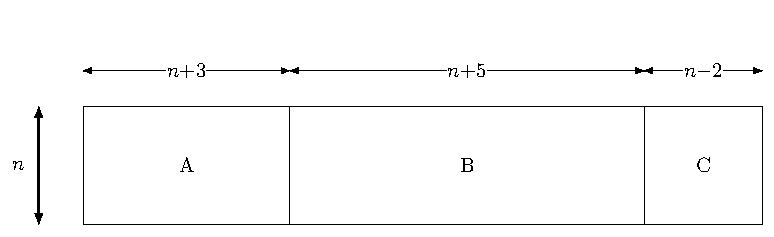
\includegraphics[height=5cm,page=1]{sprint-18-figure}
\end{center}


\fbox{\phantom{ANSWER}}

\begin{answer}
Label the figure with the lengths we find. 
\begin{center}
\includegraphics[height=5cm,page=2]{sprint-18-figure}
\end{center}
The measure of angle ABE is $60^{\circ}$ ($180-90=60$), so triangle ABE is a $(90,60,30)$ triangle. Any $(90,60,30)$ triangle has legs in multiples of $1$ and $\sqrt{3}$, with hypotenuse $2$. Here the hypotenuse is AB $=6$, so the legs must be AE $=3\sqrt{3}$ and (the shorter leg) BE $=3$. Since F is the midpoint, BF $=3/2$. Applying the Pythagorean theorem to triangle CBF gives:
\begin{align*}
\text{CF} 
& = \sqrt{6^2 + \left(\frac{3}{2}\right)^2} \\[2ex]
& = \sqrt{\frac{4 \times 36 + 9}{4}} \\[2ex]
& = \sqrt{\frac{153}{4}} \\[2ex]
& = \frac{3\sqrt{17}}{2}
\end{align*}
Matching this to $\dfrac{a\sqrt{b}}{c}$ gives $a=3$, $b=17$, $c=2$ and $a+b+c=22$. 

\subsection*{The $\mathbf{(90,60,30)}$ Triangle}
The lengths of the $(90,60,30)$ triangle can be found by applying the Pythagorean theorem. Consider triangle ABC shown below, with a right-angle at A.
\begin{center}
\includegraphics[height=7cm,page=3]{sprint-18-figure}
\end{center}
Apply the Pythagorean theorems: 
\begin{align*}
\text{AB}^2 + \text{AC}^2 & = \text{BC}^2
\end{align*}
Since the measure of angle ACB ($60^{\circ}$) is twice the measure of angle ABC ($30^{\circ}$), it follows that $\text{BC}=2\text{AC}$. Substituting into the equation above yields:
\begin{align*}
\text{AB}^2 + \text{AC}^2 
  & = 4\text{AC}^2 \\
\Rightarrow\qquad
\text{AB} 
  & = \sqrt{3}\text{AC}
\end{align*}
So, for instance: 
$\text{AC}=1$, $\text{BC}=2$, $\text{AB}=\sqrt{3}$,
as shown in the figure. 
\begin{empheq}[box={\mathbox[colback=white]}]{equation*}
    22
\end{empheq} 
\end{answer}
%%%%%%%%%%%%%%%%%%%%%%%%%%%%%%%%%%%%%%%%%%%%%%%%%%%%%%%%%%%%%%%%%%%%%%%%

\iftoggle{showAnswers}{\newpage}

%%%%%%%%%%%%%%%%%%%%%%%%%%%%%%%%%%%%%%%%%%%%%%%%%%%%%%%%%%%%%%%%%%%%%%%%
\subsection*{19.}

\nopagebreak

When $257$ is divided by $m$, the remainder is $5$. How many possible positive integer values are there for $m$? 

\fbox{\phantom{ANSWER}}

\begin{answer}
The statement may be written mathematically as
\begin{align*}
257 & = km + 5, ~\text{with}~k,m \in \mathbb{N} \\
\Rightarrow\quad
252 & = km, ~\text{with}~ m > 5 ~\text{for some}~ k > 0
\end{align*}
Clearly $m=1$ does not satisfy the conditions, since it leaves a remainder of $257$, not $5$. 
How many factors does $252$ have? How many are larger than $5$?
\begin{align*}
252 = 2^2 \times 3^2 \times 7^1
\end{align*}
The number of factors is the product of one plus the exponent on each of the prime factors:
\begin{align*}
(2+1) \times (2+1) \times (1+1) = 18
\end{align*}
Of these we remove the factors that are less than or equal to $5$, which are $1,2,3,4$. Thus,
\begin{align*}
18 - 4 = 14
\end{align*}

\begin{empheq}[box={\mathbox[colback=white]}]{equation*}
    14
\end{empheq} 
\end{answer}
%%%%%%%%%%%%%%%%%%%%%%%%%%%%%%%%%%%%%%%%%%%%%%%%%%%%%%%%%%%%%%%%%%%%%%%%

\iftoggle{showAnswers}{\newpage}

%%%%%%%%%%%%%%%%%%%%%%%%%%%%%%%%%%%%%%%%%%%%%%%%%%%%%%%%%%%%%%%%%%%%%%%%
\subsection*{20.}

\nopagebreak

In Pierre's sports league, each team plays at most one game per day. Furthermore, no team is allowed to play games on three consecutive days, nor may any team play four or more games in any five consecutive days. Under these constraints, what is the maximum number of games Pierre's team could play in a $108$-day interval?

\fbox{\phantom{ANSWER}}~games

\begin{answer}
Let $Y$ denote a day when Pierre's team plays a game and $N$ a day when the team does not play. The $108$ days can be broken down into multiple, identical $5$-day segments finished by one $3$ segment:
\begin{align*}
108 = 105 + 3 = 5 \times 21 + 3
\end{align*}
\begin{align*}
\underbrace{YYNYN}_{\dfrac{3}{5}} \quad \underbrace{YYNYN}_{\dfrac{3}{5}} \quad \ldots \quad \underbrace{YYNYN}_{\dfrac{3}{5}} \quad  \underbrace{YYN}_{\dfrac{2}{3}}
\end{align*}
Adding up over all the $Y$s,
\begin{align*}
3 \times 21 + 2 = 65
\end{align*}
\begin{empheq}[box={\mathbox[colback=white]}]{equation*}
    65 ~\text{games}
\end{empheq} 
\end{answer}
%%%%%%%%%%%%%%%%%%%%%%%%%%%%%%%%%%%%%%%%%%%%%%%%%%%%%%%%%%%%%%%%%%%%%%%%

\iftoggle{showAnswers}{\newpage}

%%%%%%%%%%%%%%%%%%%%%%%%%%%%%%%%%%%%%%%%%%%%%%%%%%%%%%%%%%%%%%%%%%%%%%%%
\subsection*{21.}

\nopagebreak

What is the value of the expression shown? Express your answer as a common fraction. 
\begin{align*}
3 + \dfrac{3}{3 + \dfrac{3}{3 + \dfrac{3}{3 + \dfrac{3}{3 + \dfrac{3}{3}}}}}
\end{align*}

\begin{minipage}[b]{\linewidth}
\fbox{\phantom{ANSWER}}\\
\mbox{---------------}\\
\fbox{\phantom{ANSWER}}
\end{minipage}

\begin{answer}
Consider the sequence:
\begin{align*}
s_{n} = 3 + \dfrac{3}{s_{n-1}}
\end{align*}
where $s_{n}$ is the value of the fraction nested $n$ times, so that the fifth term $s_{5}$ is the value we are looking for. Since the nesting has only $5$ levels, we can calculate $s_{5}$ step by step:
\begin{align*}
s_{1} 
 & = 3 + \dfrac{3}{3} 
   = 4 \\
s_{2} 
 & = 3 + \dfrac{3}{s_{1}} 
   = 3 + \dfrac{3}{4}
   = \frac{15}{4} \\
s_{3} 
 & = 3 + \dfrac{3}{s_{2}} 
   = 3 + \dfrac{3 \times 4}{15}
   = \frac{45+12}{15}
   = \frac{57}{15} 
   = \frac{19}{5} \\
s_{4} 
 & = 3 + \dfrac{3}{s_{3}} 
   = 3 + \dfrac{3 \times 5}{19}
   = \frac{57+15}{19}
   = \frac{72}{19} \\
s_{5} 
 & = 3 + \dfrac{3}{s_{4}} 
   = 3 + \dfrac{3 \times 19}{72}
   = \frac{216+57}{72}
   = \frac{3\times72+3\times19}{3 \times 24}
   = \frac{91}{24}
\end{align*}
In the above we made use of $57=3\times19$ and $216=3\times72$ several times. 
\begin{empheq}[box={\mathbox[colback=white]}]{equation*}
    \frac{91}{24}
\end{empheq} 
\end{answer}
%%%%%%%%%%%%%%%%%%%%%%%%%%%%%%%%%%%%%%%%%%%%%%%%%%%%%%%%%%%%%%%%%%%%%%%%

\iftoggle{showAnswers}{\newpage}

%%%%%%%%%%%%%%%%%%%%%%%%%%%%%%%%%%%%%%%%%%%%%%%%%%%%%%%%%%%%%%%%%%%%%%%%
\subsection*{22.}

\nopagebreak

The equation $x^2 + y^2 -2x + 4y = -4$ is true for how many ordered pairs of integers $(x,y)$?

\fbox{\phantom{ANSWER}}~

\begin{answer}
We can re-express the equation in terms of the squares $(x-1)^2$ and $(y+2)^2$:
\begin{align*}
x^2 + y^2 -2x + 4y & = -4 \\
x^2 - 2x + 1 + y^2 + 4y + 4 & = - 4 + 1 + 4 \\
(x-1)^2 + (y+2)^2 & = 1
\end{align*}
This is the equation of a circle of radius $1$ centered at point $(1,-2)$. The small size of the radius suggests the circle is not going to go through many pairs of integers. Clearly each of the squared expression must be between $0$ and $1$. For instance, if $(x-1)^2=0$, then $(y+2)^2=1$ and vice versa. Collecting these facts yields $4$ solutions:
\begin{align*}
(x,y) \in \{(1,-3), (1,-1), (0,-2), (2,-2) \}
\end{align*}
\begin{empheq}[box={\mathbox[colback=white]}]{equation*}
    4
\end{empheq} 
\end{answer}
%%%%%%%%%%%%%%%%%%%%%%%%%%%%%%%%%%%%%%%%%%%%%%%%%%%%%%%%%%%%%%%%%%%%%%%%

\iftoggle{showAnswers}{\newpage}

%%%%%%%%%%%%%%%%%%%%%%%%%%%%%%%%%%%%%%%%%%%%%%%%%%%%%%%%%%%%%%%%%%%%%%%%
\subsection*{23.}

\nopagebreak

If $n$ is an integer such that the value of the expression $4n+5n+6n+7n$ is a four-digit positive integer containing each of the digits $4$, $5$, $6$, and $7$, what is the greatest possible value of $n$? 

\fbox{\phantom{ANSWER}}

\begin{answer}
A number expressible as $4n+5n+6n+7n=22n$ contains the digits $4,5,6,7$ in some arrangement, e.g. $4567$, with no repeating digits. Thus, whatever that number is, it must have $22$ as a factor, and therefore $2$ and $11$ as well. So it must be even, which implies that it must end with either $4$ or $6$. To use the fact that $11$ is a factor is harder. If we denote the digits of the number as $abcd$, a well-known divisibility-by-$11$ rule states that there must be some integer $k$ (positive or negative) such that
\begin{align*}
(a + c) - (b + d) = 11k
\end{align*}
However, the largest difference (in absolute value) is $(6+7)-(4+5)=4$, so $k$ cannot exceed $0$, that is $k=0$ and
\begin{align*}
a + c = b + d
\end{align*}
Since the $4$ digits are consecutive, the $(a,c)$ and $(b,d)$ pairs must satisfy
\begin{align*}
4 + 7 = 5 + 6
\end{align*}
so that $(a,c)$ is either $(4,7)$ or $(7,4)$ or $(5,6)$ or $(6,5)$, and likewise for $(b,d)$. Putting that information together yields only two candidates:
\begin{align*}
abcd = a7c4  \quad\text{or}\quad abcd = a5c6 
\end{align*}
The greatest of these integers is $7546$. This yields the value of $n$ by division:
\begin{align*}
n = \frac{7546}{22} = 343
\end{align*}
\begin{empheq}[box={\mathbox[colback=white]}]{equation*}
    343
\end{empheq} 
\end{answer}
%%%%%%%%%%%%%%%%%%%%%%%%%%%%%%%%%%%%%%%%%%%%%%%%%%%%%%%%%%%%%%%%%%%%%%%%

\iftoggle{showAnswers}{\newpage}

%%%%%%%%%%%%%%%%%%%%%%%%%%%%%%%%%%%%%%%%%%%%%%%%%%%%%%%%%%%%%%%%%%%%%%%%
\subsection*{24.}

\nopagebreak

If $x$ and $y$ are positive numbers with $x-y=12$ and $\sqrt[3]{x}-\sqrt[3]{y}=2$, what is value of $xy$? Express your answer as a common fraction.

\begin{minipage}[b]{\linewidth}
\fbox{\phantom{ANSWER}}\\
\mbox{---------------}\\
\fbox{\phantom{ANSWER}}
\end{minipage}

\begin{answer}
These expressions reminds us of the well-known $a^3-b^3=(a-b)(a^2+ab+b^2)$, but with cubic-roots instead of cubes. A simple transformation can bring our beloved cubes back. Let $a=\sqrt[3]{x}$ and $b=\sqrt[3]{y}$, implying $x=a^3$ and $y=b^3$. Rewriting the given conditions in terms of $a$ and $b$ yields:
\begin{align*}
\sqrt[3]{x} - \sqrt[3]{y} = a - b & = 2 \\
x - y = a^3 - b^3 & = 12 
\end{align*}
Now substitute, factorize, simplify:
\begin{align*}
x - y 
  & = 12 \\
a^3 - b^3 
  & = 12 \\ 
\underbrace{(a-b)}(a^2 + ab + b^2) 
  & = 12 \\
2 \quad (a^2 + ab + b^2) 
  & = 12 \\
a^2 + ab + b^2
  & = 6
\end{align*}
One approach now is to substitute $b=a-2$ and solve for $a$. That is overkill because the question asks for the product $xy=a^3b^3$, not for $x$ and $y$ separately, but let's do it anyway to see what happens:
\begin{align*}
a^2 + a(a-2) + (a-2)^2 & = 6 \\
3a^2 - 6a & = 2 \\ 
3(a-1)^2 - 3 & = 2\\
(a-1)^2 - \frac{5}{3} & = 0\\
\left(a-1-\sqrt{\frac{5}{3}}\right) \left(a-1+\sqrt{\frac{5}{3}}\right) & = 0\\
\end{align*}
and so $a$ equals either $1+\sqrt{\frac{5}{3}}$ or $1-\sqrt{\frac{5}{3}}$. From this we need to get $b=a-2$ and cube both expressions. Tedious and error prone. So let's go back and think more. We are looking for the product $ab$, which appears in this expression:
\begin{align*}
a^2 + ab + b^2 = 6
\end{align*} 
This looks a little like $(a+b)^2$, which reminds us that the product $ab$ will appear if I square $(a+b)$ or $(a-b)$ (or any sum involving $a$ and $b$. But we have just the sum!
\begin{align*}
a - b = 2 \\
(a - b)^2 = 4 \\
a^2 -2ab + b^2 = 4
\end{align*} 
If only we could get rid of the $a^2$ and $b^2$ \ldots. Or wait! Let's subtract these:
\begin{align*}
a^2 + ab + b^2 = 6 \\
a^2 -2ab + b^2 = 4 \\
\cline{1-2} 
3ab = 2
\end{align*} 
and thus 
\begin{align*}
ab & = \frac{2}{3}\\
\quad \Rightarrow 
xy & = a^3 b^3 = (ab)^3 = \left(\frac{2}{3}\right)^3 = \frac{8}{27}
\end{align*} 
\begin{empheq}[box={\mathbox[colback=white]}]{equation*}
    \frac{8}{27}
\end{empheq} 
\end{answer}
%%%%%%%%%%%%%%%%%%%%%%%%%%%%%%%%%%%%%%%%%%%%%%%%%%%%%%%%%%%%%%%%%%%%%%%%

\iftoggle{showAnswers}{\newpage}

%%%%%%%%%%%%%%%%%%%%%%%%%%%%%%%%%%%%%%%%%%%%%%%%%%%%%%%%%%%%%%%%%%%%%%%%
\subsection*{25.}

\nopagebreak

In a certain game, Players $1$ through $5$ take turns rolling a standard six-sided die, beginning with Player $1$. If a six is rolled, that player wins. If any other number is rolled, the die is given to the player whose number corresponds to the number rolled, even if that is the player whose turn it currently is. What is the probability that Player $1$ wins? Express your answer as a common fraction.

\begin{minipage}[b]{\linewidth}
\fbox{\phantom{ANSWER}}\\
\mbox{---------------}\\
\fbox{\phantom{ANSWER}}
\end{minipage}

\begin{answer}
Player 1 rolls
\quad
\begin{align*}
\scaleleftright[1.75ex]{<}{
  \begin{array}{c}
    6 \hspace{34pt} \text{with probability} \quad \dfrac{1}{6} \quad \text{and wins with probability} \quad 1 \\[3ex]
    1\ldots5 \quad \text{with probability} \quad \dfrac{5}{6} \quad \text{and wins with probability} \quad \dfrac{1}{5}
  \end{array}}
{}
\end{align*}

And thus: 
\begin{align*}
\frac{1}{6} \times 1 + \frac{5}{6} \times \frac{1}{5}
  = \frac{1}{3}
\end{align*}
\begin{empheq}[box={\mathbox[colback=white]}]{equation*}
    \frac{1}{3}
\end{empheq} 
\end{answer}
%%%%%%%%%%%%%%%%%%%%%%%%%%%%%%%%%%%%%%%%%%%%%%%%%%%%%%%%%%%%%%%%%%%%%%%%

\iftoggle{showAnswers}{\newpage}

%%%%%%%%%%%%%%%%%%%%%%%%%%%%%%%%%%%%%%%%%%%%%%%%%%%%%%%%%%%%%%%%%%%%%%%%
\subsection*{26.}

\nopagebreak

If $t$ is a real number such that $t+1/t=3$, what is the value of $t^5+1/t^5$?

\fbox{\phantom{ANSWER}}

\begin{answer}
Raise the given expression to the power $5$ using the binomial expansion theorem:
\begin{align*}
t + \frac{1}{t} 
  & \quad=\quad 3 \\[2ex]
\left(t + \frac{1}{t}\right)^5 
  & \quad=\quad 3^5 \\[2ex]
t^5 + 5 t^4\,\frac{1}{t} + 10 t^3\,\frac{1}{t^2} + 10 t^2\,\frac{1}{t^3} + 5 t\,\frac{1}{t^4} + \frac{1}{t^5} 
  & \quad=\quad 3^5 \\[2ex]
t^5+\frac{1}{t^5} + 5 \left(t^3+\frac{1}{t^3}\right) + 10 \left(t+\frac{1}{t}\right) 
  & \quad=\quad 243
\end{align*}
Apply the binomial expansion theorem again on the power of $3$:
\begin{align*}
t + \frac{1}{t} 
  & \quad=\quad 3 \\[2ex]
\left(t + \frac{1}{t}\right)^3 
  & \quad=\quad 3^3 \\[2ex]
t^3 + 3 t^2\,\frac{1}{t} + 3 t\,\frac{1}{t^2} + \frac{1}{t^3} 
  & \quad=\quad 27 \\[2ex]
t^3+\frac{1}{t^3} + 3 \underbrace{\left(t+\frac{1}{t}\right)}_{\textstyle 3} 
  & \quad=\quad 27 \\[2ex]
t^3 + \frac{1}{t^3} 
  & \quad=\quad 18
\end{align*}
Putting it all together yields:
\begin{align*}
t^5+\frac{1}{t^5} + 5 \underbrace{\left(t^3+\frac{1}{t^3}\right)}_{\textstyle 18} + 10 \underbrace{\left(t+\frac{1}{t}\right)}_{\textstyle 3} 
  & = 243 \\
t^5 + \frac{1}{t^5} 
  & = 123
\end{align*}
\begin{empheq}[box={\mathbox[colback=white]}]{equation*}
    123
\end{empheq} 
\end{answer}
%%%%%%%%%%%%%%%%%%%%%%%%%%%%%%%%%%%%%%%%%%%%%%%%%%%%%%%%%%%%%%%%%%%%%%%%

\iftoggle{showAnswers}{\newpage}

%%%%%%%%%%%%%%%%%%%%%%%%%%%%%%%%%%%%%%%%%%%%%%%%%%%%%%%%%%%%%%%%%%%%%%%%
\subsection*{27.}

\nopagebreak

In base $b$, we have $r=0.\overline{57}_{b}$ and $3r=1.\overline{06}_{b}$. What is the value of $r$ in base ten? Express your answer as a common fraction.

\begin{minipage}[b]{\linewidth}
\fbox{\phantom{ANSWER}}\\
\mbox{---------------}\\
\fbox{\phantom{ANSWER}}
\end{minipage}

\begin{answer}
No hints provided.
\begin{empheq}[box={\mathbox[colback=white]}]{equation*}
    \frac{29}{85}
\end{empheq} 
\end{answer}
%%%%%%%%%%%%%%%%%%%%%%%%%%%%%%%%%%%%%%%%%%%%%%%%%%%%%%%%%%%%%%%%%%%%%%%%

\iftoggle{showAnswers}{\newpage}

%%%%%%%%%%%%%%%%%%%%%%%%%%%%%%%%%%%%%%%%%%%%%%%%%%%%%%%%%%%%%%%%%%%%%%%%
\subsection*{28.}

\nopagebreak

The integers from $1$ to $16$ are placed in the $16$ circles in the figure shown, with each number occurring exactly once and so that the sum of the six numbers around each hexagon is $S$. What is the greatest possible value of $S$?

\begin{center}
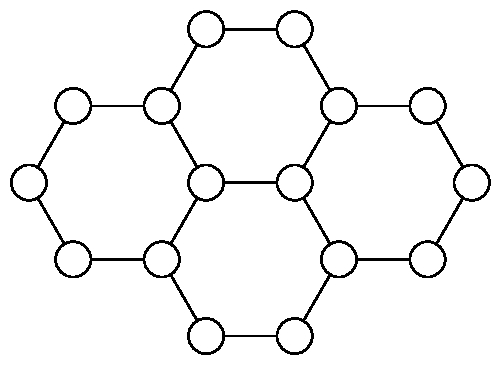
\includegraphics[height=5cm,page=1]{sprint-28-figure}
\end{center}

\begin{answer}
No hints provided.
\begin{empheq}[box={\mathbox[colback=white]}]{equation*}
    62
\end{empheq} 
\end{answer}
%%%%%%%%%%%%%%%%%%%%%%%%%%%%%%%%%%%%%%%%%%%%%%%%%%%%%%%%%%%%%%%%%%%%%%%%

\iftoggle{showAnswers}{\newpage}

%%%%%%%%%%%%%%%%%%%%%%%%%%%%%%%%%%%%%%%%%%%%%%%%%%%%%%%%%%%%%%%%%%%%%%%%
\subsection*{29.}

\nopagebreak

Marian throws a dart that lands randomly on a dartboard shaped like an isosceles trapezoid with side lengths $12$ inches, $12$ inches, $12$ inches, and $24$ inches. What is the probability that the dart is closer to the $24$-inch side than it is to any of the other three sides of the dartboard? Express your answer as a common fraction.

\begin{minipage}[b]{\linewidth}
\fbox{\phantom{ANSWER}}\\
\mbox{---------------}\\
\fbox{\phantom{ANSWER}}
\end{minipage}

\begin{answer}
No hints provided.
\begin{empheq}[box={\mathbox[colback=white]}]{equation*}
    \frac{5}{12}
\end{empheq} 
\end{answer}
%%%%%%%%%%%%%%%%%%%%%%%%%%%%%%%%%%%%%%%%%%%%%%%%%%%%%%%%%%%%%%%%%%%%%%%%

\iftoggle{showAnswers}{\newpage}

%%%%%%%%%%%%%%%%%%%%%%%%%%%%%%%%%%%%%%%%%%%%%%%%%%%%%%%%%%%%%%%%%%%%%%%%
\subsection*{30.}

\nopagebreak

For $0 \leq x \leq 1$, the function $f(x)$ satisfies the relations
\begin{align*}
f\left(\frac{x}{x+1}\right) & = \frac{f(x)}{2}\\
f(1-x) & = 1- f(x)
\end{align*}
What is the value of the expression 
\begin{align*}
f\left(\frac{2}{3}\right) + f\left(\frac{2}{5}\right) + f\left(\frac{2}{7}\right) + \ldots + f\left(\frac{2}{2n+1}\right)
\end{align*}
Express your answer as a common fraction.

\begin{minipage}[b]{\linewidth}
\fbox{\phantom{ANSWER}}\\
\mbox{---------------}\\
\fbox{\phantom{ANSWER}}
\end{minipage}

\begin{answer}
No hints provided.
\begin{empheq}[box={\mathbox[colback=white]}]{equation*}
    \frac{3}{2}
\end{empheq} 
\end{answer}
%%%%%%%%%%%%%%%%%%%%%%%%%%%%%%%%%%%%%%%%%%%%%%%%%%%%%%%%%%%%%%%%%%%%%%%%

\end{document}